\documentclass[12pt,a4paper]{book}
\usepackage[utf8]{inputenc}
%\usepackage{setspace}
\usepackage{amsmath}
\usepackage{amsfonts}
\usepackage{amssymb}
\usepackage{graphicx}
\usepackage[francais]{babel}
\usepackage[T1]{fontenc}
\usepackage{tikz,lipsum,lmodern}
\usepackage[most]{tcolorbox}
\usepackage{geometry}
\usepackage{xcolor}
\usepackage{sectsty}
\usepackage{varwidth}
\usepackage{wrapfig}
\usepackage{float}
\usepackage{capt-of}
\usepackage[export]{adjustbox}
\usepackage{graphicx} %table
\usepackage{tabularx}
\usepackage[explicit]{titlesec}
\usepackage{subcaption}
\usepackage[Lenny]{fncychap}
\usepackage{fancyhdr}
\pagestyle{fancy}
%Lenny Sonny Glenn Bjornstrup
%\chapterfont{\color{red}} 
%\sectionfont{\color{red}} 
%\subsectionfont{\color{blue}} 
%\subsubsectionfont{\color{brown}}
\geometry{top=3cm, bottom=3cm, left=2.5cm, right=2.5cm}
\title{\color{red} \textbf{Cours Tranc commun Technologie}}
\author{\bsc{Nait Lyasse} Mjid}
\date{}
%%##############################################################################
\DeclareTColorBox{Box}{ O{تعريف} O{blue}}
{title={\sffamily #1},colback=#2!5,colframe=#2,boxed title style={size=small,colback=#2!5},coltitle=black}
%%##############################################################################
\newtcbtheorem[auto counter,number within=section]{exemple}%
{\textbf{Exemple}}{enhanced jigsaw,breakable,fonttitle=\bfseries\upshape, fontupper=\slshape,
	arc=1mm, colback=white!5!white,colframe=blue!75!black}{theorem}

\newtcbtheorem[auto counter,number within=section]{definition}%
{définition}{fonttitle=\bfseries\upshape, fontupper=\slshape,
	arc=1mm, colback=green!5!white,colframe=green!75!black}{}

%%###############################################################################
%\renewcommand\thechapter{\arabic{chapter}}
\renewcommand\thesection{\Roman{section} .}
\renewcommand\thesubsection{\arabic{subsection}.}
\renewcommand\thesubsubsection{\alph{subsubsection}.}
\definecolor{titlegrammar}{RGB}{255,128,0}
\renewcommand\headrulewidth{1pt}
\renewcommand\headwidth{\linewidth}
\renewcommand\footrulewidth{1pt}
%\usepackage{fontspec}
%\setromanfont{Times New Roman}
%  \setsansfont{Arial}
%  \setmonofont[Color={0019D4}]{Courier New}
\begin{document}
	\setcounter{figure}{0}
	\setcounter{chapter}{0}
	\fancyhead[R]{Chapitre 1 : Les espèces chimiques}
	\fancyhead[L]{Partie : Chimie}
	\fancyfoot[L]{Tronc commun technologique}
	\fancyfoot[R]{Prof: Nait Lyasse Majid}
	\chapter{Les espèces chimiques
	}
	
\renewcommand{\labelitemi}{$\bullet$}	%=====================================================================================================
\textbf{\section{Notion d'espèce chimique}
\subsection{Les corps homogènes et les mélanges}
\noindent
Quel est la différence entre la composition d'un corps homogène et un corps hétérogène?
\begin{figure}[!h]
\begin{subfigure}{.5\textwidth}
  \centering
  \fbox{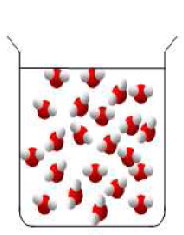
\includegraphics[width=.58\linewidth,height=.7\linewidth]{images/c1im1_2.png}}
  \caption{l'eau pure}
  \label{fig:c1im1_2}
\end{subfigure}%
\begin{subfigure}{.5\textwidth}
  \centering
  \fbox{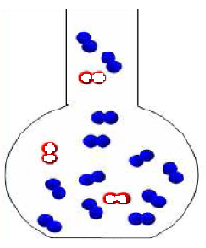
\includegraphics[width=.58\linewidth,height=.7\linewidth]{images/c1im1_1.png}}
  \caption{air}
  \label{fig:c1im1_1}
\end{subfigure}
%\caption{مكونات الماء الخالص والهواء}
\label{fig:c1im1_2}
\end{figure}
\begin{itemize}
\item $H_2O$ est constitué d'un seul type d'entités chimiques, donc l'eau est espèce chimique.
\item l'air est constitue de plusieurs espèces chimiques. donc l'air est une substance chimique.
\end{itemize}
\subsection{Espèce chimique}
\noindent
Espèce chimique est un ensemble constitué d'un seul type d'entités chimiques (corps pur),elle peut être représentée par une formule chimique ou un symbole par exemple : eau $(H_2O)$, fer $(Fe)$, glucose $(C_6H_{12}O_6)$ ...
\section{Identifications des espèces chimiques}
\subsection{Utilisation des cinq sens}
\noindent
\begin{minipage}{0.70\linewidth}
Est ce que nos organes de sens sont capables de révéler l'existence de toutes les espèces chimiques qui se trouvent dans une orange? Pour répondre à cette question,On Observe l'aspect extérieur de cette Orange, on coupe le fruit en deux, puis on le regarde, on le touche, on le sent, on le goute.\\
1- Au fur et à mesure des observations, compléter le tableau suivant :
\end{minipage}
\begin{minipage}{0.3\linewidth}
  \begin{flushright}
  \fbox{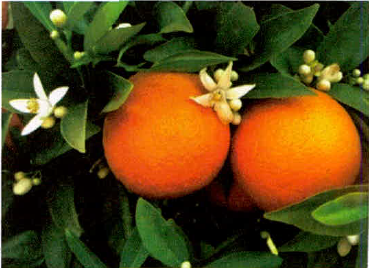
\includegraphics[width=.98\linewidth]{images/c1/im1.png}}
  \end{flushright}
\end{minipage}
% \usepackage{array} is required
\begin{tabularx}{\linewidth}{|X|>{\centering\arraybackslash}p{0.1\linewidth}|>{\centering\arraybackslash}p{0.1\linewidth}|>{\centering\arraybackslash}p{0.1\linewidth}|>{\centering\arraybackslash}p{0.1\linewidth}|>{\centering\arraybackslash}p{0.1\linewidth}|}
\hline 
 & Vue & Toucher & Gout & Odorat & Ouie \\ 
\hline 
est colorée &  &  &  &  &  \\ 
\hline 
est odorante &  &  &  &  &  \\ 
\hline 
contient de l'eau &  &  &  &  &  \\ 
\hline 
contient des gaz &  &  &  &  &  \\ 
\hline 
est acide &  &  &  &  &  \\ 
\hline 
est sucrée &  &  &  &  &  \\ 
\hline 
est salée &  &  &  &  &  \\ 
\hline 
est grasse &  &  &  &  &  \\ 
\hline 
\end{tabularx} \\
2- L'utilisation des sens est-elle suffisante pour identifier tous les constituants d'une orange?
\\Les sens ne peuvent pas identifier tous les constituants du fruit.
\subsection{Réalisation de quelques tests chimiques}
\subsubsection{Test de la présence de l'eau}
\noindent
\begin{itemize}
\item A l'aide d'une spatule, on place un peu de sulfate de cuivre anhydre de couleur pratiquement blanche dans une coupelle, puis on verse quelques gouttes de l'eau distillée sur la poudre. on observe alors que le sulfate de cuivre anhydre devient bleu au contact de l'eau.\\
\item On répand avec une spatule un peu de sulfate de cuivre anhydre sur la pulpe d'une orange, on observe alors que le sulfate de cuivre anhydre prend la couleur bleue.
\end{itemize}
\begin{figure}[!h]
\begin{subfigure}{.5\textwidth}
  \centering
  \fbox{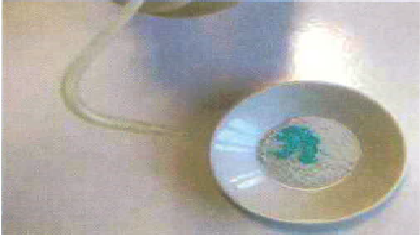
\includegraphics[width=.6\linewidth]{images/c1/im2_1.png}}
  \caption{l'eau pure}
  \label{fig:c1im1_2}
\end{subfigure}%
\begin{subfigure}{.5\textwidth}
  \centering
  \fbox{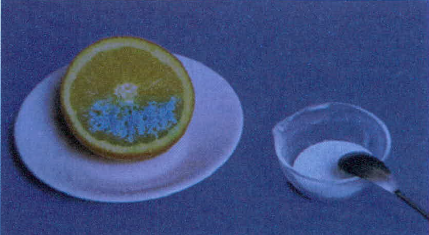
\includegraphics[width=.6\linewidth]{images/c1/im2_2.png}}
  \caption{Orange}
  \label{fig:c1im1_1}
\end{subfigure}
\label{fig:c1im1_2}
\end{figure}
\noindent
Que peut-on conclure?
\\l'orange contient de l'eau
\subsubsection{Test de l'acidité}
On verse environ 20 mL de jus d'orange dans un bécher, et on mesure le pH de la solution à l'aide d'un stylo pH-mètre.\\
\begin{center}
\fbox{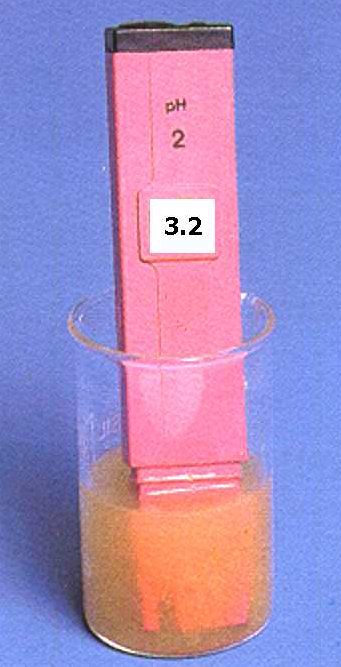
\includegraphics[width=.2\linewidth]{images/c1/im3_1.png}}
\end{center}
Relever la valeur affichée par le stylo pH-mètre. que peut-on conclure?\\
la valeur affichée par le stylo pH-mètre est pH = 3.2, donc le jus d'orange est acide.
\begin{Box}[Remarque][titlegrammar]
\begin{itemize}
\item On peut testé l'acidité à l'aide d'une indicateur coloré bleu de bromothymol (BBT).
\begin{center}
\fbox{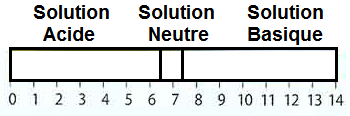
\includegraphics[width=.6\linewidth]{images/c1/im5_2.png}}
\end{center}
\item On peut aussi utilisé le papier pH.
\begin{center}
\fbox{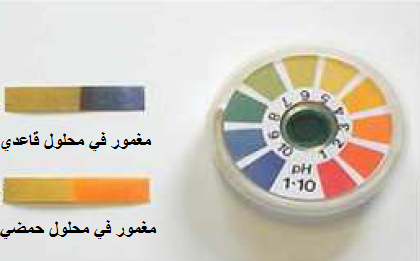
\includegraphics[width=.6\linewidth]{images/c1/im3_2.png}}
\end{center}
\end{itemize}
\end{Box}
\subsubsection{Test la présence de glucose}
\noindent
la liqueur de fehling est une solution de couleur bleue. Chauffée en présence de glucose, elle donne un précipité rouge brique.\\
Dans un tube à essai, on introduit 5 mL de jus d'orange et 2 mL de liqueur de fehling, puis on chauffe le mélange.
\begin{figure}[!h]
\begin{subfigure}{.5\textwidth}
  \centering
  \fbox{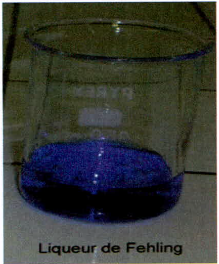
\includegraphics[width=.59\linewidth]{images/c1/im4_1.png}}
  \caption{Liqueur de fehling}
  \label{fig:c1im1_2}
\end{subfigure}%
\begin{subfigure}{.5\textwidth}
  \centering
  \fbox{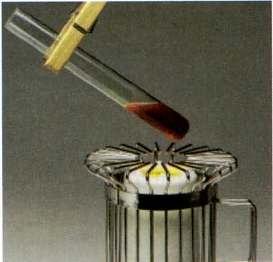
\includegraphics[width=.73\linewidth]{images/c1/im4_2.png}}
  \caption{jus d'orange}
  \label{fig:c1im1_1}
\end{subfigure}
\label{fig:c1im1_2}
\end{figure}\\
Observer et conclure.\\
il y a formation d'un précipité rouge brique, le jus d'orange contient du glucose.
\subsubsection{Test la présence de l'amidon}
\noindent
Le réactif qui permet de tester la présence de l'amidon est l'eau iodée. En effet une solution de diode devient bleu-noire en présence de l'amidon.
\begin{center}
\fbox{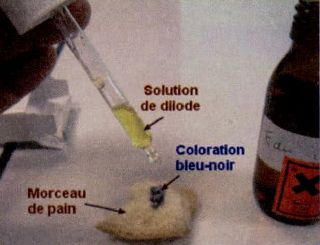
\includegraphics[width=.7\linewidth]{images/c1/im5.png}}
\end{center}
\section{Classification des substances}
\subsection{Substance naturelle}
\noindent
Une substance naturelle est une substance qui existe dans la nature.\\
Exemples :\\
Le lait ; Le miel ; L'eau minérale ; l'huile d'olive ; la laine ; le coton ...
\subsection{Substance synthétique}
\noindent
Une Substance synthétique est une substance fabriquée par l'Homme.\\
Exemples :\\
Les matière plastique ; les peintures ; les médicaments et de nombreux textiles ...
\subsection{Substance artificielle}
\noindent
Une Substance artificielle est une substance synthétique qui n'existe pas dans la nature.\\
Exemples :\\
Le nylon ; le polystyrène...}
\end{document}

